\documentclass[MS,synopsis]{iitmdiss}
\usepackage{times}
\usepackage{t1enc}

%\usepackage[dvips]{graphicx}
%\usepackage[hypertex]{hyperref} % hyperlinks for references.
\usepackage{hyperref} % hyperlinks for references.
\usepackage{amsmath} % easier math formulae, align, subequations \ldots
\usepackage{graphicx}
\usepackage{epstopdf}

\usepackage{macros}

\title{A Study on Online Sequential Learning using Bandits}

\author{Subhojyoti Mukherjee}

\date{December 2017}
\department{COMPUTER SCIENCE AND ENGINEERING}


\begin{document}

%\nocite{*}
\maketitle

\newpage
\
\thispagestyle{empty}
\clearpage

% The main text will follow from this point so set the page numbering
% to arabic from here on.
\pagenumbering{arabic}
\setcounter{page}{1}

%\afterpage{\null\newpage}


\section{Introduction}
\label{synopsis:intro}
In today's world, artificial intelligence has proved to be a game-changer in designing agents that interact with an evolving environment and make decisions on the fly. The main goal of artificial intelligence is to design artificial agents that make dynamic decisions in an evolving environment. In pursuit of these, the agent can be thought of as making a series of sequential decisions by interacting with the dynamic environment which provides it with some sort of feedback after every decision which the agent incorporates into its decision-making strategy to formulate the next decision to be made. A large number of problems in science and engineering, robotics and game playing, resource management, financial portfolio management, medical treatment design, ad placement, website optimization and packet routing can be modeled as sequential decision-making under uncertainty. Many of these real-world interesting
sequential decision-making problems can be formulated as reinforcement learning (RL) problems (\citep{bertsekas1996neuro}, \citep{sutton1998reinforcement}). In an RL problem, an agent interacts with a dynamic, stochastic, and unknown environment, with the goal of finding an action-selection strategy or policy that optimizes some long-term performance measure. Every time when the agent interacts with the environment it receives a signal/reward from the environment based on which it modifies its policy. The agent learns to optimize the choice of actions over several time steps which is learned from the sequences of data that it receives from the environment. This is the crux of online sequential learning. 

    This is in contrast to supervised learning methods that deal with labeled data which are independently and identically distributed (i.i.d.) samples from the considered domain and train some classifier on the entire training dataset to learn the pattern of this distribution to predict the labels of future samples (test dataset) with the assumption that it is sampled from the same domain. In contrast to this, an RL agent learns from the samples that are collected from the trajectories generated by its sequential interaction with the system. For an RL agent, the trajectory consists of a series of sequential interactions whereby it transitions from one state to another following some dynamics intrinsic to the environment while collecting the reward till some stopping condition is reached. This is known as an episode. Here, for an action $i_t$ taken by the agent at the $t$-th timestep, the agent transitions from its current state denoted by $S_{i,t}$ to state $S_{i,t+1}$ and observes the reward $X_{i,t}$. An illustrative image depicting the reinforcement learning scenario is shown in Figure \ref{fig:rl}.

\begin{figure}[!th]
\begin{center}
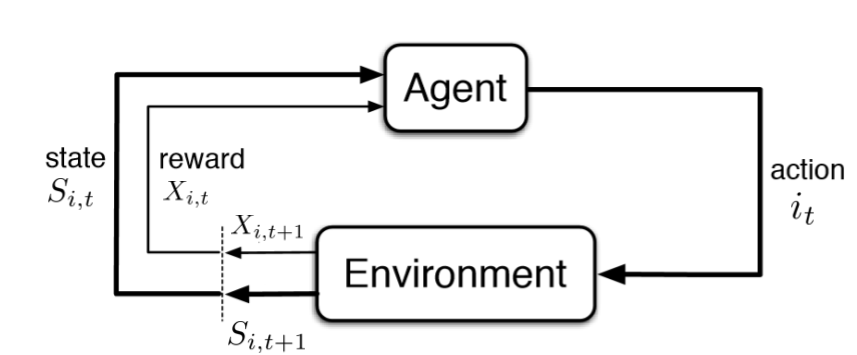
\includegraphics[scale=0.3]{synopsis/img/RL1.png}
\caption{Reinforcement Learning}
\label{fig:rl}
\end{center}
\end{figure}

Now, for a single-step interaction, i.e., when the episode terminates after a single transition, the problem is captured by the multi-armed bandit (MAB) model. Infact the MAB model can be considered as a single looping state when the agent after taking an action, and observing the reward transitions back to the same state. That single looping state consist of several finite number of actions which are called as arms.

	The name bandit originated from the concept of casino slot machine where there are levers which are termed as arms and the learner can pull one lever and observe the reward associated with that arm which is sampled from a distribution associated with the specific arm. This game is repeated $T$ times and the goal of the learner is to maximize its profit. 
	
%	There are multiple reasons to study the interesting area of bandits. First of all, bandits are the cornerstone of understanding the general reinforcement learning area. Infact, bandits helps us to understand the idea of \textit{exploration-exploitation} dilemma which is the basis to build full, multi-state, general reinforcement learning ideas. Secondly, as stated in \citet{maillard2011apprentissage}, even $50$ years after \cite{robbins1952some} introduced the first idea of bandits, there are many interesting and fruitful areas where bandit concept can be extended in both practical and theoretical terms. Finally, there are several real-life industrial applications ranging from recommendation systems, game theory to anomaly detection where bandit applications have been found to perform exceptionally well. All of these forces us to delve deep into a systemic research of bandits.
    
    
%To express an RL problem more formally, we have to define the idea of Markov Decision Process (MDP) which consists of states, actions, transition probabilities, and rewards which in turn helps in deciding the strategy to be followed by the agent. 

%An MDP consists of states


\section{Motivation}
\label{synopsis:motivation}

The MAB model fits very well in various real-world scenarios that can be modeled as sequential decision-making problems. Some of which are mentioned as follows:-
\begin{enumerate}
\item \emph{Online Shop Domain:} In the online shop domain \citep{ghavamzadeh2015bayesian}, a retailer aims to maximize profit by sequentially suggesting products to online shopping customers. In this scenario, at every timestep, the retailer displays an item to a customer from a pool of items which has the highest probability of being selected by the customer. The episode ends when the customer selects or does not select a product (which will be considered as a loss to the retailer). This feedback is incorporated by the learner as a feedback from the environment and it modifies its policy for the next suggestion. This process is repeated till a pre-specified number of times with the retailer gathering valuable information regarding the customer from this behaviour and modifying its policy to display other items to different customers.
\item \emph{Medical Treatment Design:} Another interesting domain that MAB model was first studied was for the medical treatment design \citep{thompson1933likelihood},\citep{thompson1935theory}. Here at every timestep, the learner chooses to administer one out of several treatments sequentially on a stream of patients who are suffering from the same ailment (say). Let's also assume that there is a single treatment which will be able to alleviate the patients from their disease. Here, the episode ends when the patient responds well or does not respond well to the treatment whereby the learner modifies its policy for the suggestion to the next patient. The goal of the learner is to quickly converge on the best treatment so that whenever a new patient comes with the same ailment, the learner can suggest the best treatment which can relive the patient of its ailment with a high probability.
\item \emph{Financial Portfolio Management:} In financial portfolio management MAB models can also be used. Here, the learner is faced with the choice of selecting the most profitable stock option out of several stock options. The simplest strategy where we can employ a bandit model is this; at the start of every trading session the learner suggests a stock to purchase worth Re $1$, while at the closing of the trading session it sells off the stock to witness its value after a day's trading. The  profit recorded is treated as the reward revealed by the environment and the learner modifies its policy for the next day. Let's assume that no new stock options are being introduced over the considered time horizon and there is a single best stock option which if selected for perpetuity will always give the best returns. Then, the goal of the learner is reduced to identifying the best stock option as quickly as possible. 
\item \emph{Product Selection:} A company wants to introduce a new product in market and there is a clear separation of the test phase from the commercialization phase. In this case the company tries to minimize the loss it might incur in the commercialization phase by testing as much as possible in the test phase. So from the several variants of the product that are in the test phase the learning learner must suggest the product variant(s) whose qualities are above a particular threshold $\tau$ at the end of the test phase that have the highest probability of minimizing loss in the commercialization phase. A similar problem has been discussed for single best product variant identification without threshold in \citet{bubeck2011pure}. 
\item \emph{Mobile Phone Channel Allocation:} Another similar problem as above concerns channel allocation for mobile phone communications \citep{audibert2009exploration}. Here there is a clear separation between the allocation phase and communication phase whereby in the allocation phase a learner has to explore as many channels as possible to suggest the best possible set of channel(s) whose qualities are above a particular threshold $\tau$. The threshold may depend on the subscription level of the customer such that with higher subscription the customer is allowed better channel(s) with the $\tau$ set high. Each evaluation of a channel is noisy and the learning algorithm must come up with the best possible set of suggestions within a very small  number of attempts.
\item \emph{Anomaly Detection and Classification:} MABs can also be used for anomaly detection where the goal is to seek out extreme values in the data. Anomalies may not always be naturally concentrated which was shown in  \citet{steinwart2005classification}. To implement a MAB model the best possible way is to define a cut-off level $\tau$ and classify the samples above this level $\tau$ as anomalous along with a tolerance factor which gives it a degree of flexibility. Such an approach has already been mentioned in \citet{streeter2006selecting} and further studied in \citet{locatelli2016optimal}.
\end{enumerate}


%	In all the above examples the MAB model performs well mainly because all of them suffer from \textit{exploration-exploitation dilemma}. This is characterized by action-selection choice faced by the learner where it must decide whether to stay with the action yielding highest reward till now or to explore newer actions which might be more profitable in the long run. MAB's are suited for such scenarios because 
%\begin{enumerate}
%\item They are easy to implement.
%\item The switch between exploration and exploitation is more well defined theoretically.
%\item They perform well empirically.
%\end{enumerate}


\section{Objectives and Scope of Thesis}
\label{synopsis:objThesis}
The main objectives of the thesis are as follows:-
\begin{enumerate}
\item The first objective of this thesis is to study the area of stochastic multi-armed bandit (SMAB) and how to minimize cumulative regret in this setup. We intend to give strong gap-dependent and gap-independent regret guarantees in the SMAB setting. We also intend to provide algorithm in the SMAB setting that outperforms the current state-of-the-art algorithms in this setting.

\item The second objective of this thesis is to study the area of thresholding bandit problem (TBP) setting where the goal is to minimize the expected loss at the end of a fixed budget provided as input. We intend to provide strong guarantees with respect to expected loss and also propose algorithm that does not require any problem complexity as an input. We also intend to provide strong empirical evaluations of the algorithm proposed for the TBP setting.

%\item The third objective of this thesis is to study the area of piecewise stochastic bandit where again the goal is to minimize the cumulative regret. We intend to provide strong algorithms that can adapt to this environment and performs well empirically.  
\end{enumerate}

\section{Contributions of Thesis}
\label{synopsis:contriThesis}
The main contributions of the thesis are as follows:-
\begin{enumerate}
\item We proposed a novel algorithm for the stochastic multi-armed bandit (MAB) problem. Our proposed Efficient UCB Variance method, referred to as EUCBV is an arm elimination algorithm based on UCB-Improved and UCBV strategy which takes into account the empirical variance of the arms and along with aggressive exploration factors eliminate sub-optimal arms. Through a theoretical analysis, we establish that EUCBV achieves a better gap-dependent regret upper bound than UCB-Improved, MOSS, UCB1, and UCBV algorithms. EUCBV enjoys an order optimal gap-independent regret bound same as that of OCUCB and MOSS, and better than UCB-Improved, UCB1 and UCBV. Empirically, in several considered environments EUCBV outperforms most of the state-of-the-art algorithms. 

\item We proposed the Augmented-UCB (AugUCB) algorithm for a fixed-budget version of the thresholding bandit problem (TBP), where the objective is to identify a set of arms whose quality is above a threshold. A key feature of AugUCB is that it uses both mean and variance estimates to eliminate arms that have been sufficiently explored. This is the first algorithm to employ such an approach for the considered TBP. Furthermore, in numerical evaluations we establish in several considered environments that AugUCB outperforms all the algorithms that does not take into consideration the variance of the arms in their action selection strategy.

%\item We proposed a general framework of bandit algorithms that combines change-point detection algorithm with aggregation of expert strategies in order to define efficient pulling strategies in context of the piecewise stochastic  distributions. The algorithms that we proposed for the piecewise stochastic setting are actively adaptive algorithms which performs very similarly to the oracle algorithm which has access to the changepoints and suffers no additional delay in adapting to the changing environment. 
\end{enumerate}
 

%\section{Outline of the Thesis}
%\label{synopsis:outline}
%In this chapter, we gave an overview of the various types of bandits available in the literature and also discussed about the main objectives of the thesis and our contributions. In this section, we give a general outline of the thesis that is to follow. In chapter \ref{chap:SMAB} we give a detailed overview of the stochastic multi-armed bandit model and the latest available algorithms in this setting. In the next chapter \ref{chap:EUCBV} we introduce our algorithm Efficient UCB Variance (EUCBV) for the stochastic multi-armed bandit model. We give theoretical guarantees on the performance of EUCBV and also show in numerical simulations that it indeed performs very well as compared to the state-of-the-art algorithms. In the subsequent chapter \ref{chap:tbandit1} we introduce a new variant of pure exploration multi-armed stochastic bandit called the thresholding bandit problem. We analyze the connections between thresholding bandit problem and pure exploration problem and also discuss several existing algorithms in both the settings that are relevant to carefully analyze the thresholding bandit problem. Then in chapter \ref{chap:tbandit2} we introduce our solution for the thresholding bandit problem, called the Augemented UCB (AugUCB) algorithm. We analyze our algorithm AugUCB and derive theoretical guarantees for it as well as show in numerical experiments that it indeed outperforms several state-of-the-art algorithms in the thresholding bandit setting. Finally, in chapter \ref{chap:psbandit} we introduce the piecewise-stochastic bandit model which is a new variant that strides between the stochastic and adversarial setting. We discuss extensively on this setting and also provide our solution to this setting and show in numerical simulations that our solution is very close to the optimal solution. 
%

\section{Summary of the Research Work}

We divided the research work done into two parts, in the first part we study the stochastic multi-armed bandit setting and propose an order optimal algorithm for this setting. In the second part we study the thresholding bandit problem and propose our solution to this problem. All these have been briefly discussed below.

%and in the third part we study the piecewise stochastic bandit setting and propose  our algorithm for this setting which beats several state-of-the-art algorithms.

\subsection{Efficient UCB Variance: An almost optimal algorithm in Stochastic Multi-Armed Bandit setting}

%\subsubsection{Introduction}
%In this part, we look at the stochastic multi-armed bandit (SMAB) setting and discussed how it is important in the general reinforcement learning setup. We also look at the various state-of-the-art algorithms in the literature for the SMAB setting and discuss the advantages and disadvantages of them. The regret bounds that have been proven for the said algorithms have also been discussed at length and their confidence intervals have also been compared against each other. Also in this part, we provide our solution to the SMAB setting which achieves an almost order-optimal regret bound. 

In this part, we deal with the stochastic multi-armed bandit (SMAB) setting. In its classical form, stochastic MABs represent a sequential learning problem where a learner is exposed to a finite set of actions (or arms) and needs to choose one of the actions at each timestep. After choosing (or pulling) an arm the learner receives a reward, which is conceptualized as an independent random draw from stationary distribution associated with the selected arm. Also, note that in SMAB, the distribution associated with each arm is fixed throughout the entire duration of the horizon denoted by $T$. 

%This SMAB formulation is shown in algorithm \ref{alg:SMAB}.
%
%\begin{algorithm}[!th]
%\caption{SMAB formulation}
%\label{alg:SMAB}
%\begin{algorithmic}
%\State {\bf Input:} Time horizon $T$, $K$ number of arms with unknown parameters of reward distribution
%\State \For{ each timestep $t=1,2,\ldots, T$}
%\State The learner chooses an arm $i\in\A$, where $\A$ is the set of arms and $|\A|=K$.
%\State The learner observes the reward $X_{i,t}\sim^{i.i.d} D_{i}$ where, $D_{i}$ is the distribution associated with the arm $i$. 
%\State \EndFor
%\end{algorithmic}
%\end{algorithm}

In SMAB setting, the learner seeks to identify the optimal arm as quickly as possible to maximize its rewards. In the pursuit of this, the learner faces the task of balancing exploitation and exploration. In other words, should the learner pull the arm which currently has the best-known estimates (exploit) or explores arms more thoroughly to ensure that a correct decision is being made. This is termed as the \textit{exploration-exploitation dilemma}, one of the fundamental challenges of reinforcement learning. The objective of the learner in the SMAB setting is to maximize his rewards or in other words, to minimize the cumulative regret, which is defined as follows:
\begin{align*}
R_{T}=r^{*}T - \sum_{i=1}^{K} r_{i}n_{i}(T),
\end{align*}
where $T$ is the number of timesteps, and  $z_{i}(T)$ is the number of times the algorithm has chosen arm $i$ up to timestep $T$.
The expected regret of an algorithm after $T$ timesteps can be written as,
\begin{align*}
\E[R_{T}]= \sum_{i=1}^{K} \E[n_i (T)] \Delta_i,
\end{align*}
where $\Delta_{i}=r^{*}-r_{i}$ is the gap between the means of the optimal arm and the $i$-th arm. 


%In the theoretical analysis of each algorithm, we try to obtain bounds on this cumulative regret. 

%These bounds can be both asymptotic or for a finite horizon. Again, these regret bounds can be either gap-dependent or gap-independent bounds. 
%
%\begin{enumerate}
%\item\textbf{Asymptotic regret bounds:} These type of regret bounds are valid for a large horizon $T$ tending to infinity. In other words, if the guarantees of these bounds to be held true then an infinite number of samples needs to be collected.
%
%\item\textbf{Finite horizon regret bounds:} These type of regret bounds are valid for a finite horizon when a limited number of samples are allowed to be collected. Note, that the knowledge of horizon may or may not be known to the learner.
%
%\item\textbf{Gap-Dependent regret bounds:} In gap-dependent or problem dependent regret bounds the regret is obtained as a measure of the gap $\Delta_{i}=r^{*}-r_{i}$ for an arm $i\in\A$ along with the time horizon and number of arms. It is so called because the regret bound depends explicitly on the means of the arms considered for that environment along with the stated assumptions on the distribution.
%
%\item\textbf{Gap-Independent regret bounds:} In gap-independent regret bound the regret does not contain the gaps and is stated explicitly in terms of the number of arms and the horizon. This is because the regret depends only on the distributional assumption, but not on the means of the arms considered. In fact, gap-independent regret bounds point to something more general and informative. These type of bounds actually give us the maximum possible regret such that no matter what is the policy, there will be an environment on which the policy achieves almost the same regret as the gap-independent regret upper bound. This leads to the notion of minimax regret.
%
%\item\textbf{Minimax regret bounds:} For a finite horizon $T$, $K$ number of arms, for all set of possible policies $\pi_{T,K}$ over $T$ and $K$ and all possible environment class $\mathcal{E}$ the minimax regret is given by,
%\begin{align*}
%R_T(\mathcal{E})=\inf_{\pi\in\pi_{T,K}}\sup_{E\in\mathcal{E}}R_T(\pi,E).
%\end{align*}
%
%Hence, this value is independent of any specific choice of a policy $\pi$ but only depends on $T$, $K$ and $\mathcal{E}$ where the dependence on $K$ is hidden in $\mathcal{E}$.
%\end{enumerate}


\subsubsection{Contributions}

We propose the Efficient-UCB-Variance (henceforth referred to as EUCBV) algorithm for the stochastic MAB setting. EUCBV combines the approach of UCB-Improved \citep{auer2010ucb} , CCB \citep{liu2016modification} and UCBV \citep{audibert2009exploration} algorithms. EUCBV, by virtue of taking into account the empirical variance of the arms, exploration parameters  and non-uniform arm selection (as opposed to UCB-Improved), performs significantly better than the existing algorithms in the stochastic MAB setting. EUCBV outperforms UCBV which also takes into account empirical variance but is less powerful than EUCBV because of the usage of exploration regulatory factor by EUCBV. Also, we carefully design the confidence interval term with the variance estimates along with the pulls allocated to each arm to balance the risk of eliminating the optimal arm against excessive optimism. Theoretically we refine the analysis of \citet{auer2010ucb} and prove that for $T\geq K^{2.4}$ our algorithm is order optimal and achieves a worst case gap-independent regret bound of $O\left( \sqrt{KT} \right)$ which is same as that of MOSS \citep{audibert2009minimax} and OCUCB \citep{lattimore2015optimally} but better than that of UCBV, UCB1 \citep{auer2002finite} and UCB-Improved. Here, $K$ is the total number of arms and $T$ is the total number of available timesteps,  termed as horizon. Also, the gap-dependent regret bound of EUCBV is better than UCB1, UCB-Improved and MOSS but is poorer than OCUCB. However, EUCBV's gap-dependent bound matches OCUCB in the worst case scenario when all the gaps are equal. Through our theoretical analysis we establish the exact values of the exploration parameters for the best performance of EUCBV. Our proof technique is highly generic and can be easily extended to other MAB settings. An illustrative table containing the bounds is provided in Table \ref{tab:comp-bds}. 

\begin{table}[t]
\caption{Regret upper bound of different algorithms}
\label{tab:comp-bds}
\begin{center}
\begin{tabular}{|p{5em}|p{12em}|p{7em}|}
\hline
Algorithm  &   \hspace*{1mm}Gap-Dependent & Gap-Independent \\
\hline
\hline
EUCBV		& $O\left( \dfrac{K\sigma_{\max}^{2}\log (\frac{T\Delta^2}{K})}{\Delta}\right)$ & $O\left(\sqrt{KT}\right)$\\
\hline
\hline
UCB1        & $O\left( \dfrac{K\log T}{\Delta} \right)$ & $O\left(\sqrt{KT\log T}\right)$ \\%\midrule
\hline
\hline
UCBV        & $O\left( \dfrac{K\sigma_{\max}^{2}\log T}{\Delta} \right)$ & $O\left(\sqrt{KT\log T}\right)$ \\
\hline
\hline
UCB-Imp 		& $O\left( \dfrac{K\log (T\Delta^2)}{\Delta} \right)$ & $O\left(\sqrt{KT\log K}\right)$ \\%\midrule
\hline
\hline
MOSS	     	& $O\left( \dfrac{K^2\log (T\Delta^2 /K)}{\Delta}\right)$ & $O\left(\sqrt{KT}\right)$\\%\midrule
\hline
\hline
OCUCB     	& $O\left( \dfrac{K\log (T/ H_{i})}{\Delta}\right)$ & $O\left(\sqrt{KT}\right)$\\\midrule
\end{tabular}
\end{center}
%\vspace*{-2em}
\end{table}


Empirically, we show that EUCBV, owing to its estimating the variance of the arms, exploration parameters and non-uniform arm pull, performs significantly better than MOSS, OCUCB, UCB-Improved, UCB1, UCBV, TS \citep{thompson1933likelihood},\citep{agrawal2012analysis}, BU \citep{kaufmann2012bayesian}, DMED \citep{honda2010asymptotically}, KLUCB \citep{garivier2011kl} and Median Elimination \citep{even2006action} algorithms. Note that except UCBV, TS, KLUCB and BU (the last three with Gaussian priors) all the aforementioned algorithms do not take into account the empirical variance estimates of the arms. Also, for the optimal performance of TS, KLUCB and BU one has to have the prior knowledge of the type of distribution, but EUCBV requires no such prior knowledge. EUCBV is the first arm-elimination algorithm that takes into account the variance estimates of the arm for minimizing cumulative regret and thereby answers an open question raised by \citet{auer2010ucb}, where the authors conjectured that an UCB-Improved like arm-elimination algorithm can greatly benefit by taking into consideration the variance of the arms. Also, it is the first algorithm that follows the same proof technique of UCB-Improved and achieves a gap-independent regret bound of $O\left( \sqrt{KT} \right)$ thereby, closing the gap of UCB-Improved which achieved a gap-independent regret bound of $O\left( \sqrt{KT\log K} \right)$. 

\subsubsection{The EUCBV algorithm}

\begin{algorithm}[!th]
\caption{EUCBV}
\label{alg:eucbv}
\begin{algorithmic}
\State {\bf Input:} Time horizon $T$, exploration parameters $\rho$ and $\psi$.
\State {\bf Initialization:} Set $m:=0$, $B_{0}:=\mathcal{A}$, $\epsilon_{0}:=1$, $M=\big \lfloor \frac{1}{2}\log_{2} \frac{T}{e}\big\rfloor$, $n_{0}=\big\lceil\frac{\log{(\psi T\epsilon_{0}^{2})}}{2\epsilon_{0}}\big\rceil$ and  $N_{0}=Kn_{0}$.
\State Pull each arm once
\For{$t=K+1,..,T$}	
\State Pull arm $i\in \argmax_{j\in B_{m}}\bigg\lbrace \hat{r}_{j} + \sqrt{\frac{\rho(\hat{v}_{j}+2)\log{(\psi T\epsilon_{m})}}{4 z_{j}}} \bigg\rbrace$, where $z_j$ is the number of times arm $j$ has been pulled.
%\State $t:=t+1$
\ArmElim
\State For each arm $i \in B_{m}$, remove arm $i$ from $B_{m}$ if,
\begin{align*}
 \hat{r}_{i} + & \sqrt{\frac{\rho(\hat{v}_{i}+2)\log{(\psi T\epsilon_{m})}}{4 z_{i}}}  
  < \max_{{j}\in B_{m}}\bigg\lbrace\hat{r}_{j} -\sqrt{\frac{\rho(\hat{v}_{j}+2)\log{(\psi T\epsilon_{m})}}{4 z_{j}}} \bigg\rbrace
\end{align*}
\EndArmElim
\If{$t\geq N_{m}$ and $m\leq M$}
\ResParam
\State $\epsilon_{m+1}:=\frac{\epsilon_{m}}{2}$; $B_{m+1}:=B_{m}$
\State $n_{m+1}:=\bigg\lceil\frac{\log{(\psi T\epsilon_{m+1}^{2})}}{2\epsilon_{m+1}}\bigg\rceil$
\State $N_{m+1}:=t+|B_{m+1}| n_{m+1}$; $m:=m+1$
\EndResParam
\EndIf
\State Stop if $|B_{m}|=1$ and pull ${i}\in B_{m}$ till $T$ is reached.
\EndFor
\end{algorithmic}
%\vspace*{-0.42em}
\end{algorithm}
%\vspace*{-0.42em}

\textbf{The algorithm:} Earlier round-based arm elimination algorithms like Median Elimination \citep{even2006action} and UCB-Improved mainly suffered from two basic problems: \\
\begin{inparaenum}[\bfseries(i)]
\item \textit{Initial exploration:} Both of these algorithms pull each arm equal number of times in each round, and hence waste a significant number of pulls in initial explorations. \\
\item \textit{Conservative arm-elimination:} In UCB-Improved, arms are eliminated conservatively, i.e, only after $\epsilon_{m}<\frac{\Delta_{i}}{2}$, 
% the sub-optimal arm $i$ is discarded with high probability. 
where the quantity $\epsilon_{m}$ is initialized to $1$ and halved after every round. In the worst case scenario when $K$ is large, and the gaps are uniform  ($r_{1}=r_{2}=\cdots=r_{K-1}<r^{*}$) and small this results in very high regret.\\
\end{inparaenum}
%For any round $m$ UCB-Improved pulls all arms $n_{m}=\left\lceil \frac{ 2\log(T\epsilon_{m})}{\epsilon_{m}} \right\rceil$ number of times. The quantity $\epsilon_{m}$ is initialized to $1$ and halved after every round.
\\
	The EUCBV algorithm, which is mainly based on the arm elimination technique of the UCB-Improved algorithm,  remedies these by employing exploration regulatory factor $\psi$ and arm elimination parameter $\rho$ for aggressive elimination of sub-optimal arms. Along with these, similar to CCB \citep{liu2016modification} algorithm, EUCBV uses optimistic greedy sampling whereby at every timestep it only pulls the arm with the highest upper confidence bound rather than pulling all the arms equal number of times in each round. Also, unlike the UCB-Improved, UCB1, MOSS and OCUCB algorithms (which are based on mean estimation) EUCBV employs mean and variance estimates (as in \citet{audibert2009exploration}) for arm elimination. Further, we allow for arm-elimination at every time-step, which is in contrast to the earlier work (e.g., \citet{auer2010ucb}; \citet{even2006action}) where the arm elimination takes place only at the end of the respective exploration rounds. 
	
%	An illustrative flowchart depicting the main steps is shown in Figure \ref{fig:eucbv}.
%	
%\begin{figure}[!th]
%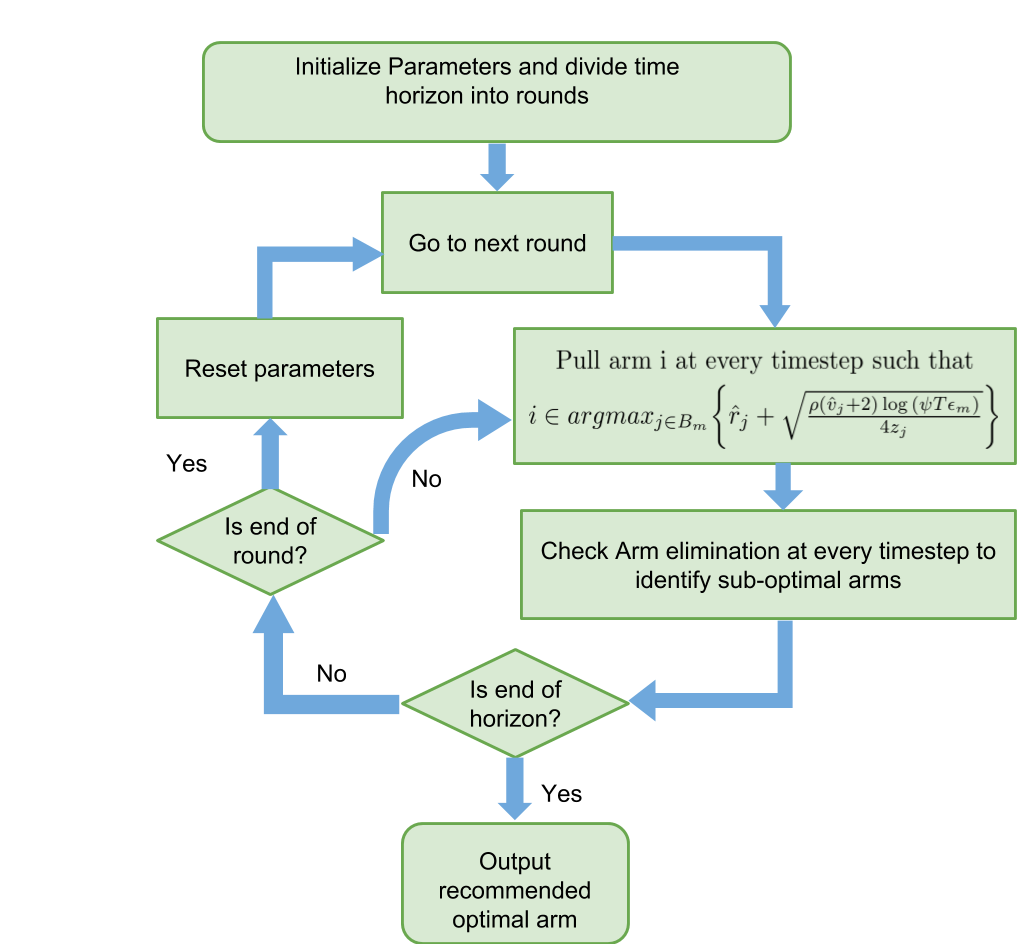
\includegraphics[scale=0.42]{synopsis/img/EUCBV_flow.png}
%\caption{Flowchart of EUCBV algorithm}
%\label{fig:eucbv}
%\end{figure}

%\subsubsection{Summary}
%
%Here, we study the Efficient UCB Variance (EUCBV) algorithm which takes into account the empirical variance of the arms and employs aggressive exploration parameters in conjunction with non-uniform arm selection to eliminate sub-optimal arms. Our theoretical analysis conclusively established that EUCBV exhibits an order-optimal gap-independent regret bound of $O\left(\sqrt{KT}\right)$. Empirically, we show that EUCBV performs superbly across diverse experimental settings and outperforms most of the bandit algorithms in an SMAB setup. Our experiments showed that EUCBV is extremely stable for large horizons and performs consistently well across different types of distributions.


\subsection{Augmented UCB for Thresholding Bandits Problem}
%In this part, we study the pure exploration MAB and thresholding bandit (TBP) setting which is a special case of combinatorial pure exploration MAB. We also study the various state-of-the-art algorithms in the literature for the pure-exploration setting and discussed the advantages and disadvantages of them. Then we look at the latest algorithm for the TBP setting. The expected loss that has been proven for the said algorithms have also been discussed at length and their exploration parameters have also been compared against each other. We provide our solution to this TBP setting which uses variance estimation to find the set of arms above the threshold. 

%In the previous part we studied the stochastic multi-armed bandit (SMAB) setting with the goal of minimizing cumulative regret. 
In this part we study another setting called pure-exploration thresholding multi-armed bandits which are unlike their traditional (exploration vs.\ exploitation)  counterparts, the SMABs, where the  objective is to minimize the cumulative regret. 
%The cumulative regret is the total loss incurred by the learner for not playing the optimal arm throughout the time horizon $T$. 
In pure-exploration problems a learning algorithm, until time $T$, can invest entirely on exploring the arms without being concerned about the loss incurred while exploring; the objective is to minimize the probability that the arm recommended at time $T$ is not the best arm.  In this chapter, we further consider a combinatorial version of the pure-exploration MAB, called the thresholding bandit problem (TBP).  Here, the learning algorithm is provided with a threshold $\tau$, and the objective, after exploring for $T$ rounds, is to  output all arms $i$ whose $r_{i}$ is above $\tau$. 
It is important to emphasize that the \emph{thresholding} bandit problem is different from the \emph{threshold} bandit setup studied in \cite{abernethy2016threshold}, where the learner receives an unit reward whenever the value of an observation is above a threshold. 

Formally, the problem we consider is the following. First, we define the set $S_{\tau}=\lbrace i\in \mathcal{A}: r_{i}\geq \tau \rbrace$. Note that, $S_\tau$ is the set of all arms whose reward mean is greater than threshold $\tau$. Let 
$S_\tau^c$ denote the complement of $S_\tau$, i.e.,  $S_{\tau}^{c}=\lbrace i\in \mathcal{A}: r_{i} < \tau \rbrace$. Next, let $\hat{S}_{\tau}=\hat{S}_{\tau}(T)\subseteq \mathcal{A}$ denote the recommendation of a learning algorithm (under consideration) after $T$ time units of exploration, while $\hat{S}_{\tau}^c$ denotes its complement. The performance of the learning agent is measured by the accuracy with which it can classify the arms into $S_{\tau}$ and $S_{\tau}^{c}$ after time horizon $T$. Equivalently, using $\mathbb{I}(E)$ to denote the indicator of an event $E$, the \emph{loss} $\mathcal{L}(T)$ is defined as
\begin{align*}
\Ls (T) = \mathbb{I}\big(\lbrace S_{\tau}\cap \hat{S}_{\tau}^{c}\neq \emptyset\rbrace    \cup    \lbrace\hat{S}_{\tau}\cap S_{\tau}^{c}\neq \emptyset\rbrace\big).
\end{align*}			
Finally, the goal of the learning agent is to minimize the expected loss:
\begin{align*}
\E[\Ls(T)] = \Pb\big(\lbrace S_{\tau}\cap \hat{S}_{\tau}^{c} \neq \emptyset \rbrace  \cup   \lbrace \hat{S}_{\tau}\cap S_{\tau}^{c} \neq \emptyset\rbrace\big).
\end{align*}
Note that the expected loss is simply the \emph{probability of mis-classification} (i.e., error), that occurs either if a good arm is rejected or a bad arm is accepted as a good one.

\subsubsection{Contributions}

We propose the Augmented UCB (AugUCB) algorithm for the fixed-budget setting of a specific combinatorial, pure-exploration, stochastic MAB called the thresholding bandit problem. AugUCB essentially combines the approach of UCB-Improved, CCB \citep{liu2016modification} and APT \citep{locatelli2016optimal} algorithms. Our algorithm takes into account the empirical variances of the arms along with mean estimates; to the best of our knowledge this is the first variance-based algorithm for the considered TBP. 
Thus, we also address an open problem discussed in \cite{auer2010ucb} of designing an algorithm that can eliminate arms based on variance estimates. In this regard, note that both CSAR \citep{chen2014combinatorial} and APT are not variance-based algorithms. 

\begin{table}[b]
\caption{AugUCB vs.\ State of the art}
\label{tab:regret-bds}
\begin{center}
\begin{tabular}{|p{2.3cm}|p{8.4cm}|}
% \toprule
\hline
Algorithm  & Upper Bound on Expected Loss \\
% \midrule
\hline
\hline
AugUCB      &$ \exp\left(- \dfrac{T}{4096 \log(K\log K)H_{\sigma,2}} + \log\left(2KT\right) \right) $ \\
\hline
\hline
UCBEV		&$\exp\left(-\dfrac{1}{512}\frac{T-2K}{H_{\sigma,1}} + \log\left(6KT\right)\right)$ \\
%\midrule
\hline
\hline
APT         &$\exp\left(-\dfrac{T}{64 H_1}+2\log((\log(T)+1)K)\right)$ \\
% \midrule
\hline
\hline
CSAR		&$\exp\left(-\dfrac{T-K}{72\log(K)H_{CSAR,2}}+2\log(K)\right)$ \\
%\midrule
\hline
%\bottomrule
\end{tabular}
\end{center}
\end{table}

Our theoretical contribution comprises proving an upper bound on the expected loss incurred by AugUCB. In Table \ref{tab:regret-bds} we compare the upper bound on the losses incurred by the various algorithms, including AugUCB. The terms $H_1, H_2$, $H_{CSAR,2}, H_{\sigma,1}$ and $H_{\sigma,2}$ represent various problem complexities. We note that, for all $K\ge 8$, we have
\begin{align*}
\log\left(K\log K\right) H_{\sigma,2} > \log(2K) H_{\sigma,2} \ge H_{\sigma,1}.
\end{align*}

Thus, it follows that the upper bound for UCBEV \citep{gabillon2011multi} is better than that for AugUCB. However, implementation of UCBEV algorithm requires $H_{\sigma,1}$ as input, whose computation is not realistic in practice. In contrast, our AugUCB algorithm requires no such complexity factor as input. Proceeding with the comparisons, we emphasize that the upper bound for  AugUCB is, in fact, not comparable with that of APT and CSAR; this is because the complexity term $H_{\sigma,2}$ is not explicitly comparable with either $H_1$ or $H_{CSAR,2}$. However, through extensive simulation experiments we find that AugUCB significantly outperforms both APT, CSAR and other non variance-based algorithms. AugUCB also outperforms UCBEV under explorations where non-optimal values of $H_{\sigma,1}$  are used. In particular, we consider experimental scenarios comprising large number of arms, with the variances of arms in $S_\tau$ being large. AugUCB, being variance based, exhibits superior performance under these settings.  

\subsubsection{The Augmented UCB algorithm}

\textbf{The algorithm:} The Augmented-UCB (AugUCB) algorithm is presented in Algorithm~\ref{alg:augucb}.
AugUCB is essentially based on the arm elimination method of the UCB-Improved \cite{auer2010ucb}, but adapted to the thresholding bandit setting proposed in \cite{locatelli2016optimal}. However, unlike the UCB improved (which is based on mean estimation) our algorithm employs \emph{variance estimates} (as in \cite{audibert2009exploration}) for arm elimination; to the best of our knowledge this is the first variance-aware  algorithm for the thresholding bandit problem. Further, we allow for arm-elimination at each time-step, which is in contrast to the earlier work (e.g., \cite{auer2010ucb,chen2014combinatorial}) where the arm elimination task is deferred to the end of the respective exploration rounds. The details are presented below.

The active set $B_{0}$ is initialized with all the arms from $\mathcal{A}$. We divide the entire budget $T$ into rounds/phases like in UCB-Improved, CCB, SAR and CSAR. At every time-step AugUCB checks for arm elimination conditions, while updating parameters at the end of each round. As suggested by \cite{liu2016modification} to make AugUCB to overcome too much early exploration, we no longer pull all the arms equal number of times in each round. Instead, we choose an arm in the active set $B_m$ that minimizes $(|\hat{r}_{i} - \tau |-2s_i)$ where $s_i  = \sqrt{\frac{\rho\psi_m (\hat{v}_{i}+1) \log ( T \epsilon_{m})}{4 n_{i}}}$ with $\rho$ being the arm elimination parameter and $\psi_{m}$ being the exploration regulatory factor.
%  in the active set $B_{m}$. 
The above condition ensures that an arm closer to the threshold $\tau$ is pulled; 
%and with suitable choice of $\rho_{\mu}$ and $\rho_v$ we can fine tune the exploration. 
parameter $\rho$ can be used to fine tune the elimination interval.
The choice of exploration factor, $\psi_m$, comes directly from \cite{audibert2010best} and \cite{bubeck2011pure} where it is  stated that in pure exploration setup, the exploring factor must be linear in $T$ (so that an exponentially small probability of error is achieved) rather than being logarithmic in $T$ (which is more suited for minimizing cumulative regret).

\begin{algorithm}[!th]
\caption{AugUCB}
\label{alg:augucb}
\begin{algorithmic}
\State {\bf Input:} Time budget $T$; parameter $\rho$; 
% $\rho_{\mu}$, $\rho_v$ 
  threshold $\tau$
\State {\bf Initialization:} $B_{0}=\mathcal{A}$; $m=0$; $\epsilon_{0}=1$;
\begin{small}
\begin{align*}
M=\left\lfloor \frac{1}{2}\log_{2} \frac{T}{e}\right\rfloor; 
\hspace{2mm}\psi_{0}=\frac{T\epsilon_{0}}{128\Big(\log(\frac{3}{16}K\log K)\Big)^2}; 
\ell_{0}=\left\lceil \frac{2\psi_0\log( T\epsilon_{0})}{\epsilon_{0}} \right\rceil;
\hspace{2mm}N_{0}=K\ell_{0}
\end{align*}
\end{small}
\State Pull each arm once
\vspace{-2mm}
\State \For{$t=K+1,..,T$}
\State Pull arm $j\in\argmin_{i\in B_{m}}\Big\lbrace |\hat{r}_{i} - \tau | - 2s_{i}\Big\rbrace$
% \State where $s_j=\sqrt{\frac{\rho\psi_{m}\hat{v}_{j}\log{( T\epsilon_{m})}}{4 n_{j}} + \frac{\rho\psi_{m} \log{(T\epsilon_{m})}}{4 n_{j}}}$
\State $t\leftarrow t+1$ 
\vspace{-4mm}
\State \For{$i\in B_m$}
\vspace{-4mm}
\State \If{$(\hat{r}_{i} + s_i  < \tau - s_i)$ or $(\hat{r}_{i} - s_i > \tau + s_i)$}
\State $B_m\leftarrow B_m\backslash\{i\}$\hspace{4mm} (Arm deletion)
\EndIf
\EndFor
\vspace{-2mm}
\State \If{$t\geq N_{m}$ and $m \leq M$}
%\ResetParam
\State \textbf{Reset Parameters}
\State $\epsilon_{m+1}\leftarrow\frac{\epsilon_{m}}{2}$; $B_{m+1} \leftarrow B_{m}$
\State $\psi_{m+1}\leftarrow \frac{T\epsilon_{m+1}}{128(\log(\frac{3}{16}K\log K))^{2}}$; $\ell_{m+1}\leftarrow\left\lceil \frac{2\psi_{m+1}\log( T\epsilon_{m+1})}{\epsilon_{m+1}} \right\rceil$
\State $N_{m+1} \leftarrow t + |B_{m+1}|\ell_{m+1}$; $m \leftarrow m+1$
%\EndResetParam
\EndIf
\EndFor
\State \textbf{Output:} $\hat{S}_{\tau}=\lbrace i: \hat{r}_{i}\geq \tau \rbrace$.
\end{algorithmic}
\end{algorithm}

%A simplified illustrative flowchart highlighting the main steps of AugUCB is provided in Figure \ref{fig:augucb}. Also note the similarity between UCB-Improved (Figure \ref{fig:ucbimp}) and AugUCB in this flowchart.
%
%\begin{figure}[!th]
%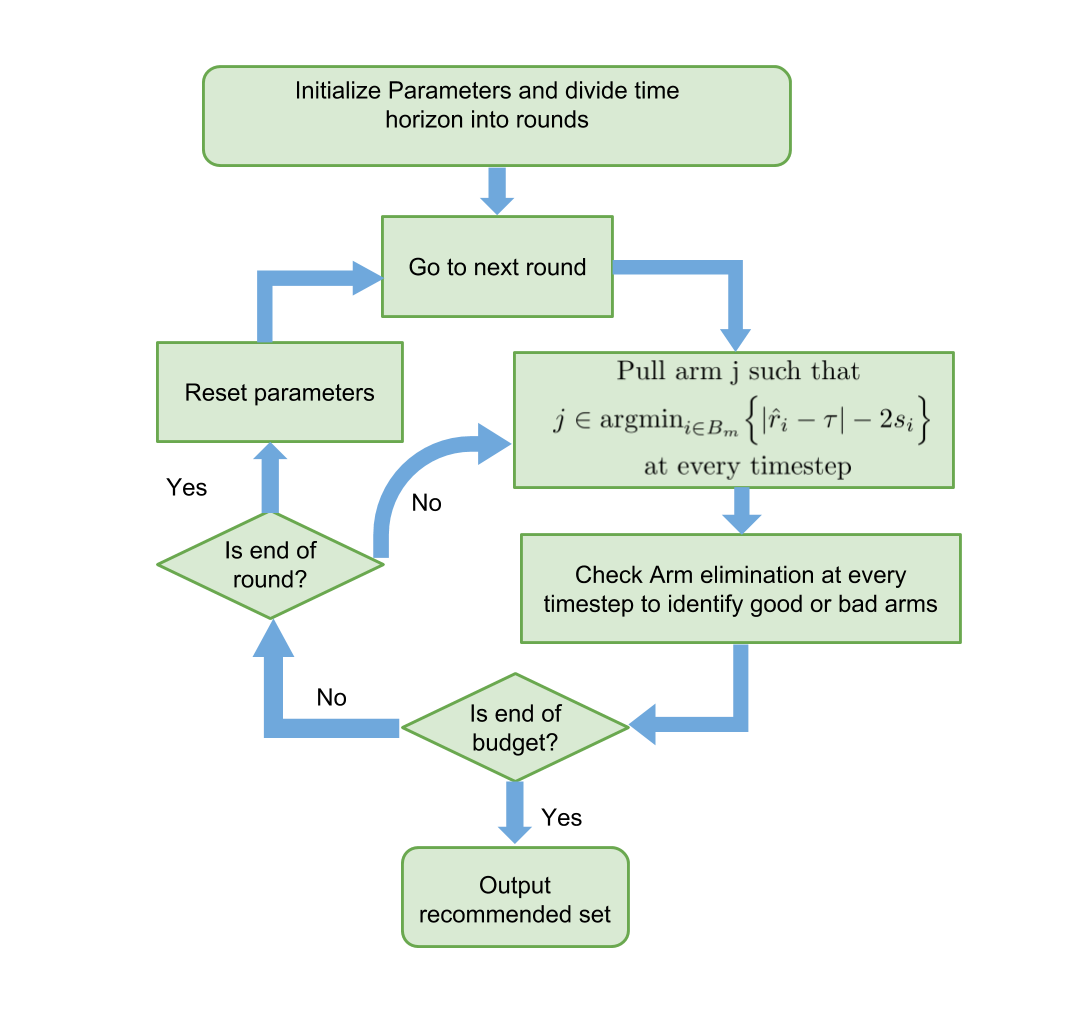
\includegraphics[scale=0.42]{synopsis/img/AugUCB_flow.png}
%\caption{Flowchart for AugUCB}
%\label{fig:augucb}
%\end{figure}
%


%\subsubsection{Summary}
%We proposed the AugUCB algorithm for a fixed-budget, pure-exploration TBP. Our algorithm employs both mean and variance estimates for arm elimination. This, to our knowledge is the first variance-based algorithm for the specific TBP that we have considered. We first prove an upper bound on the expected loss incurred by AugUCB. We then conduct simulation experiments to validate the performance of AugUCB. In comparison with APT, CSAR and other non variance-based algorithms, we find that the performance of AugUCB is significantly better. Further, the performance of AugUCB is comparable with UCBEV (which is also variance-based), although the latter exhibits a slightly better performance.  However, UCBEV is not implementable in practice as it requires computing problem complexity, $H_{\sigma,1}$, while AugUCB (requiring no such inputs) can be easily deployed in real-life scenarios.

%Also because of the said condition, like \cite{liu2016modification} we also claim that AugUCB is an anytime algorithm.



%\subsection{Improved Changepoint Detection for Piecewise Stationary Distributions}

\section{Conclusions}
\label{synopsis:Conclusions}
In this thesis, we studied two complex bandit problems, the stochastic multi-armed bandit (SMAB) with the goal of cumulative regret minimization and pure exploration stochastic thresholding bandit problem (TBP) with the goal of expected loss minimization. For the first problem, we devised a novel algorithm called Efficient UCB Variance (EUCBV) which enjoys an order optimal regret bound and performs superbly in diverse stochastic environments. In the second part, the thresholding bandit problem, we came up with the novel algorithm called Augmented UCB (AugUCB) which is the first algorithm to use variance estimation for the considered TBP setting and also empirically outperforms most of the other algorithms. 

%Finally, we studied the piecewise stochastic bandits and proposed several solutions for adaptive algorithms that detect changepoints and try to adapt accordingly.

%    There are several directions in which the work done in this thesis can be extended. Starting with the SMAB setting, there are many fundamental questions that need to be answered. Though EUCBV reached an order optimal regret bound of $80\sqrt{KT}$, still the constant associated with the bound is quite large and can be reduced by finer analysis. One avenue for future work is to remove the constraint of $T\geq K^{2.4}$ required for EUCBV to reach the order optimal regret bound. Also, EUCBV does not have any asymptotic guarantee and we do not know whether it can reach the \citet{lai1985asymptotically} asymptotic lower bound discussed in chapter \ref{chap:SMAB}. Recently another algorithm called KL-UCB++ \citep{menard2017minimax} has been proved to be both minimax optimal and asymptotically optimal. Further, EUCBV requires the knowledge of horizon as input and it will be interesting to find an anytime version of EUCBV. Similar anytime version of MOSS \citep{degenne2016anytime} and OCUCB \citep{lattimore2016regret} has also been proposed in literature.
%    
%    The thresholding bandit problem is also being intensely studied in the bandit community and there are several directions where this work can be extended. One way is to modify the APT algorithm itself and come up with a variance adaptive version of APT. This has bee recently studied in \citet{kano2017good}. Also, currently there are no lower bounds for the TBP setting considering only variance estimation and it will be interesting to derive a lower bound for this setting. Again, whereas APT is an anytime algorithm AugUCB is not anytime and it needs several modifications to obtain an anytime version of AugUCB. Further, we can also derive a gap-independent and gap-dependent bounds for AugUCB as like APT. In \citet{lattimore2015optimally} the authors showed that APT like UCB1 enjoys a gap-dependent cumulative regret bound of $O\left( \dfrac{K\log T}{\Delta^2}\right)$ and gap-independent regret bound of $O\left( \sqrt{KT\log T}\right)$.
    
    %For the piecewise stochastic bandits we were able to show empirically that the adaptive algorithms we considered are indeed more powerful than passive algorithms and further work needs to be done to derive the regret bounds for these algorithms. 
    %Specifically for CPD\ref{alg:CPD3} we find the confidence interval obtained by Laplace method as like UCB-$\delta$ algorithm\citep{abbasi2011improved} very promising and more work needs to be done in this aspect.
    
    %Finally, to summarize everything, the bandit community is actively researching several of these open problems discussed here and we hope to answer some of these problems in near future. Further, several interesting variations of the problems discussed here are also being studied such as the Contextual Thresholding Bandit problem, Combinatorial Bandit problems \citep{cesa2012combinatorial} and more powerful algorithms for changepoint detection.






%%%%%%%%%%%%%%%%%%%%%%%%%%%%%%%%%%%%%%%%%%%%%%%%%%%%%%%%%%%%
% Bibliography.

%\begin{singlespace}
%\begin{thebibliography}{10}
%\addcontentsline{toc}{section}{Bibliography}
%
%\bibitem{paper1}
%Author 1 and Author 2
%\newblock {\em Paper title}.
%\newblock Journal\ \ {\bf Volume}, Page\ \ (Year).
%\end{thebibliography}
%
%\end{singlespace}

\begin{singlespace}
\bibliographystyle{iitm}
\bibliography{refs}
\end{singlespace}



%%%%%%

\section{Proposed Contents of the Thesis}

In chapter 1 (table \ref{tab:chap1}), we discuss on Reinforcement Learning and its connection to bandits, we give an overview of the various types of bandits available in the literature and also discuss about the main objectives of the thesis and our contributions. 


%\begin{center}
\begin{table}[!th]
\begin{center}
\begin{tabular}{|p{26em}|}
\hline\\
\textbf{1. Introduction to Bandits} \\\hline
1.1 Reinforcement Learning \\
1.2 Connection between Reinforcement Learning and Bandits \\
1.3 Why study Bandits?\\
1.4 Motivation \\
1.5 Types of Information Feedback\\
1.6 Different types of Bandits\\
1.7 Objectives of Thesis\\
1.8 Contributions of Thesis\\
1.9 Outline of the Thesis\\
\hline
\end{tabular}
\end{center}
\caption{Introduction to thesis}
\label{tab:chap1}
\end{table}
%\end{center}


In chapter 2 (table \ref{tab:chap2-3}) we give a detailed overview of the stochastic multi-armed bandit setting and the latest available algorithms in this setting. In the next chapter 3 (table \ref{tab:chap2-3}) we introduce our algorithm Efficient UCB Variance (EUCBV) for the stochastic multi-armed bandit setting. We give theoretical guarantees on the performance of EUCBV and also show in numerical simulations that it indeed performs very well as compared to the state-of-the-art algorithms. 


\begin{table}[!th]
\begin{tabular}{p{16em}|p{16em}}
\hline\\
\textbf{2. Stochastic Multi-armed Bandits} & \textbf{3. Efficient UCB Variance: An almost optimal algorithm in SMAB setting}\\\hline
2.1 Introduction to SMAB & 3.1 Introduction\\
2.2 Notations and assumptions & 3.2 Our Contributions\\
2.3 Problem Definition & 3.3 Algorithm: Efficient UCB Variance\\
2.4 Motivation & 3.4 Main Results\\
2.5 Related Work in SMAB & 3.5 Proofs\\
2.6 Summary & 3.6 Experiments\\
& 3.7 Summary\\
& 3.8 Appendix B\\
\hline
\end{tabular}
\caption{Part 1. Stochastic MAB problem}
\label{tab:chap2-3}
\end{table}


In the subsequent chapter 4 (table \ref{tab:chap4-5})  we introduce a new variant of pure exploration multi-armed stochastic bandit called the thresholding bandit problem. We analyze the connections between thresholding bandit problem and pure exploration problem and also discuss several existing algorithms in both the settings that are relevant to carefully analyze the thresholding bandit problem. Then in chapter 5 (table \ref{tab:chap4-5}) we introduce our solution for the thresholding bandit problem, called the Augemented UCB (AugUCB) algorithm. We analyze our algorithm AugUCB and derive theoretical guarantees for it as well as show in numerical experiments that it indeed outperforms several state-of-the-art algorithms in the thresholding bandit setting. 


\begin{table}[!th]
\begin{tabular}{p{16em}|p{16em}}
\hline\\
\textbf{4. Thresholding Bandits} & \textbf{5. Augmented UCB for Thresholding Bandit Problem}\\\hline
4.1 Introduction to TBP & 5.1 Introduction\\
4.2 Notations and assumptions & 5.2 Our Contributions\\
4.3 Problem Definition & 5.3 Augmented-UCB Algorithm\\
4.4 Motivation & 5.4 Theoretical Results\\
4.5 Related Work in Pure Exploration & 5.5 Numerical Experiments\\
4.6 TBP connection to Pure Exploration & 5.6 Summary\\
4.7 Related Work in TBP &\\
4.8 Summary & \\
\hline
\end{tabular}
\caption{Part 2. Thresholding Bandit Problem}
\label{tab:chap4-5}
\end{table}

Finally, in chapter 6, we conclude with a brief discussion on the work done in the thesis and future directions. 

%(table \ref{tab:chap6})
%\begin{table}[!th]
%\begin{center}
%\begin{tabular}{|p{16em}|}
%\hline\\
%\textbf{6. Conclusion and Future Direction} \\\hline
%6.1 Conclusion and Future Direction \\
%\hline
%\end{tabular}
%\end{center}
%\caption{Conclusion and Future Direction of thesis}
%\label{tab:chap6}
%\end{table}


%Finally, in chapter \ref{chap:psbandit} we introduce the piecewise-stochastic bandit model which is a new variant that strides between the stochastic and adversarial setting. We discuss extensively on this setting and also provide our solution to this setting and show in numerical simulations that our solution is very close to the optimal solution. 


%\framebox{
%      \vbox{\vspace{2mm}
%%    \hbox to 6.28in { {\bf Improved Changepoint Detection for Piece-wise Stochastic Bandits
%%		\hfill Winter 2017} }
%       \vspace{4mm}
%       \hbox to 6.28in { {\Large \hfill Improved Changepoint Detection for Piece-wise Stochastic Bandits  \hfill} }
%       \vspace{2mm}
%       \hbox to 6.28in { {\it \hfill Subhojyoti Mukherjee, Odalric-Ambrym Maillard \hfill} }
%      \vspace{2mm}}
%   }


%The outline of the thesis is as follows:
%\begin{enumerate}
%\item Introduction to Bandits
%\item Stochastic Multi-armed Bandits
%\item Efficient UCB Variance: An almost optimal algorithm in Stochastic Multi-armed Bandit setting
%\item Thresholding Bandits
%\item Augmented UCB for Thresholding Bandits Problem
%%\item Improved Changepoint Detection for Piecewise Stationary Distributions
%\item Conclusion and Future Direction
%\end{enumerate}


%\vskip 4cm
%%%%%%
\section{Publications}
\subsection{Papers in Refereed Journals}
%\begin{enumerate}
%\item Title \\
%	{\bf Author 1}, Author 2...\\
%	{\it Journal title.}, {\bf Volume}, Page (Year)
%\end{enumerate}
%\begin{enumerate}
%\item Subhojyoti Mukherjee, K.P.~Naveen, Nandan Sudarsanam, and Balaraman Ravindran, ``\textit{Thresholding Bandit with Augmented UCB}'', \newblock{\em Proceedings of the Twenty-Sixth International Joint Conference on
%               Artificial Intelligence, {IJCAI} 2017, Melbourne, Australia, August
%               19-25, 2017,2515-2521}, main conference track.
%\item Subhojyoti Mukherjee, K.P.~Naveen, Nandan Sudarsanam, and Balaraman Ravindran, ``\textit{Efficient UCBV: An Almost Optimal Algorithm using Variance Estimates}'', \newblock{\em To appear in Proceedings of the Thirty-Second Association for the Advancement of Artificial Intelligence, {AAAI} 2018, New Orleans, Louisiana, USA, February 2-7}, main conference track.
%\end{enumerate}


\subsection{Presentations in Conferences}
\begin{enumerate}
\item Presented {\em Thresholding Bandit with Augmented UCB} at the {\bf Twenty-Sixth International Joint Conference on Artificial Intelligence, {IJCAI} 2017}, Melbourne, Australia, August 19-25.
\item To present {\em Efficient UCBV: An Almost Optimal Algorithm using Variance Estimates} at the {\bf Thirty-Second Association for the Advancement of Artificial Intelligence, {AAAI} 2018}, New Orleans, Louisiana, USA, February 2-7.
\end{enumerate} 
\end{document}

